\documentclass[12pt,reqno]{amsart}
%\usepackage[margin=1in]{geometry}
\usepackage{tcolorbox}
\usepackage{amssymb}
\usepackage{amsthm}
\usepackage{amsmath}
\usepackage{amssymb}
\usepackage{mathrsfs}
\usepackage{centernot}
\usepackage{lastpage}
\usepackage{fancyhdr}
\usepackage{accents}
\usepackage{tasks}
\usepackage{graphicx}
\usepackage{natbib}
\usepackage{tabularx}
\usepackage{multirow}
\usepackage{booktabs}
\usepackage{hyperref}
\usepackage{bm}
\usepackage{float}
\theoremstyle{plain}
\usepackage{multicol}
\usepackage{enumitem,kantlipsum}

% 加上浮水印
%\usepackage{wallpaper}
%\CenterWallPaper{.180}{../qsnake-logo.jpg}


\linespread{1.2}
\parindent = 0pt
\pagestyle{fancy}
\setlength{\parindent}{0pt}
%\everymath{\displaystyle}
%new area
%\usepackage[utf8]{inputenc}
%\usepackage{CJKutf8}
%\xeCJKsetup{AutoFakeBold=true, AutoFakeSlant=true}

% 設定頭部
\fancyhead[L]{Midterm} % 左邊頭部清空
\fancyhead[C]{} % 中間頭部清空
\fancyhead[R]{} % 右邊頭部顯示頁碼

% Adjust the footer as desired:
\fancyfoot[L]{} % Left footer: Empty.
\fancyfoot[C]{\thepage} % Center footer: Empty.
\fancyfoot[R]{} % Right footer: Empty.



% we will modify sections, subsections and sub subsections
\RequirePackage{titlesec}
% Modification of section 
\titleformat{\section}[block]{\normalsize\bfseries\filcenter}{\thesection.}{.3cm}{} 


% modification of subsection and sub sub section
\titleformat{\subsection}[runin]{\bfseries}{ \thesubsection.}
{1mm}{}[.\quad]
\titleformat{\subsubsection}[runin]{\bfseries\itshape}{ \thesubsubsection.}
{1mm}{}[.\quad]

\newenvironment{solution}
  {\renewcommand\qedsymbol{$\blacksquare$}
  \begin{proof}[Solution]}
  {\end{proof}}
\renewcommand\qedsymbol{$\blacksquare$}

\newcommand{\ubar}[1]{\underaccent{\bar}{#1}}

%%%%%%%%%%%%%%%%%%%%%%%%%%%%%% Textclass specific LaTeX commands.
%\theoremstyle{plain}
%\newtheorem{thm}{\protect\theoremname}[section]
\newtheorem{thm}{\textbf{Theroem}}[section]
\newtheorem{cor}[thm]{Corollary}
\newtheorem{lmma}[thm]{Lemma}
\newtheorem*{defn}{\underline{Definition}}
\newtheorem*{prop*}{Proposition}
\newtheorem*{ex*}{Example}
\newtheorem*{sol*}{Solution}
\newtheorem*{cor*}{Corollary}
\newtheorem*{thm*}{Theorem}
\newtheorem*{lmma*}{Lemma}
\newtheorem*{rmk*}{Remark}
\newtheorem*{pf*}{\underline{\textbf{Proof\ }}}

%%%%%%%%%%%%%%%%%%%%%%%%%%%%%% User specified LaTeX commands.
\renewcommand{\P}{\mathscr{P}}
\newcommand{\B}{\mathscr{B}}
\newcommand{\A}{\mathscr{A}}
\newcommand{\C}{\mathbb{C}}
\newcommand{\CC}{\mathscr{C}}
\newcommand{\R}{\mathbb{R}}
\newcommand{\Q}{\mathbb{Q}}
\newcommand{\Z}{\mathbb{Z}}
\newcommand{\N}{\mathbb{N}}
\newcommand{\X}{\mathcal{X}}
\newcommand{\T}{\mathscr{T}}
\newcommand{\arbuni}{\bigcup_{\alpha\in I}}
\newcommand{\finint}{\bigcap_{i=1}^n}
\newcommand{\Ua}{{\textsc{U}_\alpha}}
\newcommand{\Ui}{\textsc{U}_i}
\newcommand{\pair}[2]{\left( \,#1\,,\,#2\,\right) }
\newcommand{\dint}[2]{\int_{#1}^{#2}}
\newcommand{\sett}[1]{\left\{ \,#1 \,\right\}}
\newcommand{\linearcombination}[2]{#1_1#2_1+\cdots+#1_n#2_n}
\newcommand{\slinearcombination}[1]{#1_1+\cdots+#1_n}
\newcommand{\spann}[1]{\text{span($#1$)}}
\newcommand{\sub}[1]{\text{sup}}
\newcommand{\inn}[1]{\left< #1 \right>}
\newcommand{\kernal}[1]{Ker(#1)}
\newcommand{\image}[1]{Im(#1)}
\newcommand{\norm}[1]{\parallel #1 \parallel}
\newcommand{\dia}[0]{\text{dia}}
\newcommand{\marking}[1]{\text{\color{red} #1}}
%%%%%%%%%%%%%%%%%%%%%%%%%%%%%%

\begin{document}

\title{Probability}

\author{QSnake Edition}

\maketitle

\subsection*{1. Review}$ $

\begin{defn}$ $
	\begin{enumerate}[wide, label = $\bullet$]
		\item Two events $A$ and $B$ are called mutually exclusive if $A \cap B = \emptyset$
		\item Events $A_1,A_2,A_3,\cdots$ are said to be mutually exclusive if they are pairwise mutually exclusive. That is, if $A_i \cap A_j = \emptyset$ whenever $i \neq j$.
	\end{enumerate}
\end{defn}

\begin{thm*}$ $
	\begin{enumerate}[wide,label = $\bullet$]
		\item $P(A) = 1 - P(A')$
		\item $P(A) \leq 1$, for any event $A$
		\item For any two event $A$ and $B$, $P(A \cup B) = P(A) + P(B) - P(A \cap B)$
		\item If $A \subset B,$ then $P(A) \leq P(B)$
		\item $P\left( \bigcup^{\infty}_{i = 1} A_i \right) \leq \sum^{\infty}_{i = 1}P(A_i)$ If $A_1,\cdots$ is a sequence of events
		\item If $A_1,A_2,\cdots,A_k$ are events, then $P(\bigcap_{i=1}^{k}A_i) \geq 1 - \sum_{i=1}^kP(A_i')$ 
	\end{enumerate}
\end{thm*}

\begin{proof}
	By axiom of probability.
\end{proof}

\begin{defn}
	The conditional probability of an event $A$, given the event $B$, is defined by 
	
	$$P(A~|~B) = \frac{P(A \cap B)}{P(B)}$$
	
	if $P(B) \neq 0$
\end{defn}

\begin{thm*}
	For any events $A$ and $B$,
	
	$$P(A \cap B) = P(B)P(A~|~B) = P(A)P(B~|~A)$$
\end{thm*}

\begin{thm*}[Not talk in class]
	If $B_1,\cdots,B_k$ is a collection of mutually exclusive and exhaustive events, then for any event $A$
	
	$$P(A) = \sum^{k}_{i = 1}P(B_i)P(A~|~B_i)$$
\end{thm*}

\textbf{Note.} exhaustive events:  A collection of event which union is sample space.

\begin{thm*}[Not talk in class]
	If $B_1,\cdots,B_k$ is mutually exclusive and exhaustive events, then for any event $A$ and each $j = 1,\cdots,k$
	
	$$P(B_j ~|~ A) = \dfrac{P(B_j)P(A~|~B_j)}{\sum^{k}_{i=1}P(B_i)P(A~|~B_i)} \left(  = \dfrac{P(A \cap B_j)}{P(A)}\right)$$
\end{thm*}

\begin{defn}
	Two events $A$ and $B$ are called independent events if
	
	$$P(A \cap B) = P(A)P(B)$$
	
	Otherwise, $A$ and $B$ are called dependent event
\end{defn}

\begin{thm*}
	If $A$ and $B$ are events such that $P(A) > 0$ and $P(B) > 0$, and $A$ and $B$ are independent, we get
	
	$$P(A \cap B) = P(A)P(B) \Leftrightarrow P(A~|~B) = P(A) \Leftrightarrow P(B~|~A) = P(B)$$
\end{thm*}

\begin{thm*}[Not talk in class]
	\begin{eqnarray*}
		P(A \cap B) &=& P(A)P(B)\\
		\Leftrightarrow P(A' \cap B) &=& P(A')P(B)\\
		\Leftrightarrow P(A \cap B') &=& P(A)P(B')\\ 
		\Leftrightarrow P(A' \cap B') &=& P(A')P(B')
	\end{eqnarray*}
\end{thm*}


\begin{defn}
	The $k$ events $A_1,\cdots,A_k$ are said to b independent or mutually independent if for every $j = 2,3,\cdots ,k$ and every subset of distinct indices $i_1,i_2,\cdots,i_j$
	
	$$P(A_{i1} \cap A_{i2} \cap \cdots \cap A_{ij}) = P(A_{i1})P(A_{i2})\cdots P(A_{ij})$$
\end{defn}

\newpage

\subsection*{2. Discrete Random Variable Review}


\begin{defn}
	The cumulative distribution function(CDF) of a random variable $X$ is defined for any real $x$ by
	
	$$F(x) = P[X \leq x]$$
\end{defn}


\begin{thm*}
	Let $X$ be a discrete random variable with pdf $f(x)$ and CDF $F(x)$. If the possible values of $X$ are indexed in increasing order, $x_1 < x_2 < x_3 < \cdots ,$ then:
	
	\begin{enumerate}[wide,label = ($\roman*$)]
		\item $f(x_1) = F(x_i)$
		\item for any $i>1,~f(x_i) = F(x_i) - F(x_{i-1})$
		\item if $x < x_1$ then $F(x) = 0$
		\item $F(x) = \sum_{x_i \leq x}f(x_i)$
	\end{enumerate}
\end{thm*}

\begin{thm*}
	A function $F(x)$ is a CDF for some random variable $X$ if and only if it satisfies: 
	
	\begin{enumerate}[wide, label = ($\roman*$)]
		\item $\lim_{x \rightarrow -\infty}F(x) = 0$
		\item $\lim_{x \rightarrow \infty}F(x) = 1$
		\item $\lim_{h \rightarrow 0^+} F(x+h) = F(x)$
		\item $a < b$ implies $F(a) \leq F(b)$
	\end{enumerate}
\end{thm*}

\textbf{Example.} 

Suppose that the distribution function of $X$ is given by
		$$F(b) = \begin{cases}
			0 & b<0\\
			\frac{b}{4} & 0 \leq b < 1\\ 
			\frac{1}{2} + \frac{b-1}{4} & 1\ \leq b < 2\\
		 	\frac{11}{12} & 2 \leq b < 3\\
		  	1 & 3 \leq b�
		\end{cases}$$
		\begin{enumerate}
		\item Find $P\{X = i\},~i = 1,2,3$
		\item Find $P\{\frac{1}{2} < X < \frac{3}{2�}\}$
		\end{enumerate}

\newpage

\subsection*{3. Continuous Random Variables}$ $

\begin{defn}
	Let $X$ be such a random variable. We say that $X$ is a continuous random variable if there \textbf{exists a nonnegative function $f$, define for all real $x \in (- \infty,\infty)$}, having the property that for any set $B$ of real numbers,
	
	$$P \{X \in B\} = \int_Bf(x)dx$$
	
	the function $f$ is called the probability density function of the random variable $X$
\end{defn}

\textbf{Note.} $X$ will be in $B$ may be obtained by integrating the probability density function over the set $B$. Since $X$ must assume some value, $f$ must satisfy

$$1 = P\{X \in (-\infty,\infty)\} = \int^{\infty}_{-\infty}f(x)dx$$

All probability statements about $X$ can be answered in terms of $f$, and letting $B = [a,b]$, we obtain

$$P\{a \leq X \leq b\} = \int^b_af(x)dx$$

and we let $a = b$ we get

$$P\{X = a\} = \int^a_af(x)dx = 0$$

this equation states that the probability that a continuous random variable will assume any fixed value is zero. Hence, for a continuous random variable,

$$P\{X < a\}= P\{X \leq a\} = F(a) = \int^a_{\infty}f(x)dx$$

\begin{defn}
	If $X$ is a continuous random variable having probability density function $f(x)$, then expected value of $X$ is 
	
	$$E[X] = \int^{\infty}_{\infty}xf(x)dx$$
\end{defn}

\textbf{Proposition.} If $X$ is a continuous random variable with probability density function $f(x)$, then for any real-valued function $g$,

$$E[g(X)] = \int^{\infty}_{-\infty}g(x)f(x)dx$$

To proof part of this proposition $(g(x) \geq 0)$ , we will need the following lemma.(The general proof, which follows the argument in the case we present, is indicated in Theoretical Exercises $2$ and $3$.)

\begin{lmma*}
	For a nonnegative random variable $Y$.
	
	$$E[Y] = \int^{\infty}_{0}P\{Y > y\}dy$$
\end{lmma*}

\begin{proof}
	We present a proof when $Y$ is a continuous random variable with probability density function $f_Y$. We have
	
	$$\int^{\infty}_0 P\{Y > y\}dy = \int^{\infty}_{0}\int^{\infty}_{y}f_Y(x)dxdy$$
	
	where we have used the fact that $P\{Y > y\} = \int^{\infty}_yf_Y(x)dx$, and let us change it to region $D$ first.
	
	$$\int^\infty_0 \int^\infty_y f_Y(x)dxdy = \iint_D \sin (y^2)dA$$
	
	where $D = \{(x,y)~|~y<x<\infty ,~ 0 < y < \infty\}$ the picture is
	
	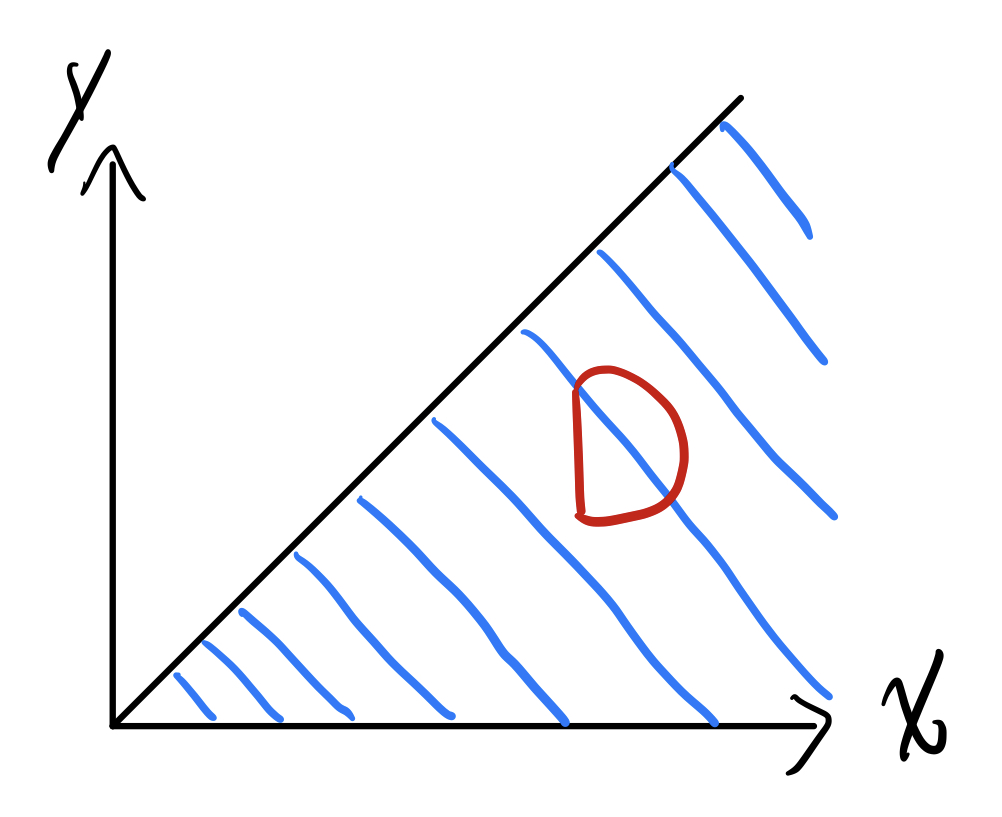
\includegraphics[scale = 0.3]{2_1.jpeg}
		
	we can consider $D$ as
	
	$$D = \{(x,y)~|~ 0 \leq x \leq \infty ,~ 0 \leq y \leq x\}$$
	
	and interchanging the order of integration in the preceding equation yields
	
	\begin{eqnarray*}
		\int^{\infty}_{0}P\{Y > y\}dy &=& \iint_D F_Y(x)dA\\
		&=& \int^{\infty}_{0}\left(\int^x_0dy\right)f_Y(x)dx\\
		&=& \int^{\infty}_0xf_Y(x)dx\\
		&=& E[Y]
	\end{eqnarray*}
\end{proof}

\textbf{Proof of Prop 2.1}

From Lemma 2.1, for any function $g$ for which $g(x) \geq 0$

\begin{eqnarray*}
	E[g(X)] &=& \int^{\infty}_0 P\{g(X) > y\}dy\\
	&=& \int^\infty_0 \int_{x:g(x)>y}f(x)dxdy\\
	&=&\int_{x:g(x)>0}\int^{g(x)}_{0}dyf(x)dx\\
	&=& \int_{x:g(x)>0}g(x)f(x)dx
\end{eqnarray*}

which completes the proof




\begin{cor*}
	If $a$ and $b$ are constants, then
	
	$$E[aX + b] = aE[X] + b$$
\end{cor*}


\newpage
\subsection*{3. Uniform Random Variable}$ $

\begin{defn}
	A random variable is said to be uniformly distributed over the interval $(0,1)$ if its probability density function is given by
	
	$$f(x) = \begin{cases}
		1 & 0 < x < 1\\
		0 & \text{otherwise}
	\end{cases}$$
	
	and in general,  we say that $X$ is a uniform random variable on the interval $(\alpha,\beta)$ if the probability density function of $X$ is given by
	
	$$f(x) = \begin{cases}
		\dfrac{1}{\beta - \alpha} & \text{if } \alpha < x < \beta \\
		0 & \text{otherwise}
	\end{cases}$$
	
	We usy $X \sim Uniform(\alpha,\beta)$
\end{defn}

\textbf{Exercise.} Let $X$ be uniformly distributed over $(\alpha , \beta)$. Find $E[X]$ and $Var(X)$

\begin{eqnarray*}
	E[X] &=& \int^{\infty}_{-\infty}xf(x)dx\\
	&=& \int^{\beta}_{\alpha} \dfrac{x}{\beta - \alpha}dx\\
	&=& \dfrac{\beta^2 - \alpha^2}{2(\beta - \alpha)}\\
	&=& \dfrac{\beta + \alpha}{2}
\end{eqnarray*}

the variance be the homework, try it yourself.

\newpage

\subsection*{4. Normal Random Variables}

\begin{defn}
	We say that $X$ is a normal random variable, or simply that $X$ is normally distributed, with parameters $\mu$ and $\sigma^2$ if the density of $X$ is given by

	$$f(x) = \dfrac{1}{\sqrt{2\pi}\sigma}e^{-(x - \mu)^2 / 2\sigma^2} \text{\hspace{20pt}} -\infty < x < \infty$$
	
	and we will usually write $X \sim N(\mu,\sigma^2)$
\end{defn}



Proof $f(x)$ is indeed a probability density function
\begin{proof}
	To prove that $f(x)$ is indeed a probability density function, we need to show that
	
	$$\dfrac{1}{\sqrt{2\pi}\sigma}\int^\infty_{-\infty}e^{-(x - \mu)^2/2\sigma^2}dx = 1$$
	
	Making the substitution $y = (x - \mu)/\sigma$, we see that
	
	$$\dfrac{1}{\sqrt{2\pi}\sigma}\int^\infty_{-\infty}e^{-(x-\mu)^2/2\sigma^2}dx = \dfrac{1}{\sqrt{2\pi}}\int^{\infty}_{-\infty}e^{-y^2/2}dy$$
	
	Hence, we must show that $$\int^{\infty}_{-\infty}e^{-y^2/2}dy = \sqrt{2\pi}$$
	
	Toward this end, let $I = \int^\infty_{-\infty}e^{-y^2/2}dy$. Then 
	
	\begin{eqnarray*}
		I^2 &=& \int^{\infty}_{-\infty}e^{-y^2/2}dy\int^{\infty}_{-\infty}e^{-x^2/2}dx\\
		&=& 2\pi \int^{\infty}_{0} re^{-r^2/2}dr\\
		&=& -2\pi e^{-r^2/2}|^{\infty}_{0}\\
		&=& 2\pi
	\end{eqnarray*}
	
	Hence, $I = \sqrt{2\pi}$, and the result is proved.
\end{proof}

\textbf{Note.} 

If $X$ is normally distributed with parameters $\mu$ and $\sigma^2$, then $Y = aX + b$ is normally distributed with parameters $a\mu + b$ and $a^2\sigma^2$

\begin{proof}
	Suppose $a > 0$. Let $F_Y$ denote the cumulative distribution function of $Y$. Then
	
	\begin{eqnarray*}
		F_Y(x) &=& P\{Y \leq x\}\\
		&=& P\{aX + b \leq x\}\\
		&=&P\left\{X \leq \dfrac{x - b}{a}\right\}\\
		&=&F_X\left(\dfrac{x-b}{a}\right)
	\end{eqnarray*}
	
	and by differentiation, the density function of $Y$ is then
	
	\begin{eqnarray*}
		f_Y(x) &=& \dfrac{1}{a}f_X\left(\dfrac{x-b}{a}\right)\\
		&=& \dfrac{1}{\sqrt{2\pi}a\sigma}exp\left\{ -\left(\dfrac{x - b}{a} - \mu / 2 \sigma^2\right)\right\}\\
		&=& \dfrac{1}{\sqrt{2\pi}a\sigma}exp\{-(x - b - a\mu)^2/2(a\sigma)^2\}
	\end{eqnarray*}
	
	which shows that $Y$ is normal with parameters $a\mu + b$ and $a^2\sigma^2$
\end{proof}

\textbf{Exercise.} Find $E[X]$ and $Var(X)$ when $X$ is a normal random variable with parameters $\mu$ and $\sigma^2$

\textbf{Note.} If $X$ is normally distributed with parameters $\mu$ and $\sigma^2$, then $Z = (X - \mu)/\sigma$ is normally distributed with parameters $0$ and $1$. Such a random variable is said to be a standard, or a unit normal random variable.

\begin{proof}
	Start by finding the mean and variance  of the standard normal random variable $Z = (X - \mu)/\sigma$/ We have
	\begin{eqnarray*}
		E[Z] &=& \int^\infty_{-\infty}xf_Z(x)dx\\
		&=& \dfrac{1}{\sqrt{2\pi}}\int^\infty_{-\infty}xe^{-x^2/2}dx\\
		&=& -\dfrac{1}{\sqrt{2\pi}}e^{-x^2/2}|^{\infty}_{-\infty}\\
		&=&0
	\end{eqnarray*}
	
	Thus,
	
	\begin{eqnarray*}
		Var(Z) &=& E[Z^2]\\
		&=& \dfrac{1}{\sqrt{2\pi}}\int^{\infty}_{\infty}x^2e^{-x^2/2}dx
	\end{eqnarray*}
	
	Integration by parts (with $u = x$ and $dv = xe^{-x^2/2}$) now gives
	
	\begin{eqnarray*}
		Var(Z) &=& \dfrac{1}{\sqrt{2\pi}}\left(-e^{-x^2/2}|^{\infty}_{-\infty} +  \int^{\infty}_{-\infty}e^{-x^2/2}dx  \right) \\
		&=& \dfrac{1}{\sqrt{2\pi}}\int^{\infty}_{\infty}e^{-x^2/2}dx\\
		&=& 1
	\end{eqnarray*}
\end{proof}

Because $X = \mu + \sigma Z$, the preceding yields the results

$$E[X] = \mu + \sigma E[Z] = \mu \text{ and } Var (X) = \sigma^2Var(Z) = \sigma^2$$

\begin{defn}
	If $X \sim N(\mu,\sigma^2)$ then $X = \sigma Z + \mu$ where $Z \sim N(0,1)$. We call $Z$ a standard normal random variable.
\end{defn}

\begin{defn}
	It is customary to denote the cumulative distribution function of a standard normal random variable by $\Phi(x)$. That is ,
	
	$$\Phi(x) = \dfrac{1}{\sqrt{2\pi}}\int^x_{-\infty}e^{-y^2/2}dy$$
\end{defn}

%\textbf{The Normal Approximation to the Binomial Distribution}



\newpage

\subsection*{5. Exponential Random Variables}$ $

\begin{defn}
	A continuous random variable whose probability density function is given, for some $\lambda > 0$, by
	
	$$f(x) = \begin{cases}
		\lambda e^{-\lambda x} & \text{ if }x\geq 0\\
		0 & \text{ if } x < 0
	\end{cases}$$
	
	is said to be an exponential random variable with parameter $\lambda$. The cumulative distribution function $F(a)$ of an exponential random variable is given by
	
	\begin{eqnarray*}
		F(a) &=& P \{X \leq a\}\\
		&=& \int^a_{0} \lambda e^{-\lambda x}dx\\
		&=&-e^{-\lambda x}|^a_0\\
		&=& 1 - e^{\lambda a} \hspace{30pt} a \geq 0
	\end{eqnarray*}
\end{defn}

\textbf{Exercise.} Let $X$ be an exponential random variable with parameter $\lambda$. Calculate $E[X]$ an $Var(X)$.

\textbf{Hazard Rate Functions}

\begin{defn}
	Consider a positive continuous random variable $X$ that we interpret as being the life time of some item. Let $X$ have distribution function $F$ and density $f$. The hazard rate (sometimes called the failure rate) function $\lambda(t)$ of $F$ is defined by
	
	$$\lambda(t) = \dfrac{f(t)}{\overline{F}(t)}, \hspace{20pt} \text{where }\overline{F} = 1 - F$$
	
	Suppose now that the lifetime distribution is exponential. Then, by the memory-less property, it follows that the distribution of remaining life for a $t$-year-old item is the same as that for a new item.
	
	$$\lambda(t) = \dfrac{f(t)}{\overline{F}(t)} = \dfrac{\lambda e^{-\lambda t}}{e^{-\lambda t}} = \lambda$$
\end{defn}

\newpage

\subsection*{$\text{6.}^*$ The Gamma Distribution}

A random variable is said to have a gamma distribution with parameters $(\alpha,\lambda), \lambda > 0,\alpha > 0$, if its density function is given by

$$f(x) = \begin{cases}
	\dfrac{\lambda e^{-\lambda x}(\lambda x)^{\alpha - 1}}{\Gamma (\alpha)} & x \geq 0\\
	0 & x < 0
\end{cases}$$

where $\Gamma(\alpha) = \int^{\infty}_{0}e^{-y}y^{\alpha - 1}dy$ is called \textbf{gamma function}.

\textbf{Note}. Some times, the $\lambda$ in the equation above will be changed to $\beta$, and normally $\beta = \dfrac{1}{\lambda}$

Now, let's check the property of $\Gamma(\alpha)$, integration of $\Gamma(\alpha)$ by parts yields

\begin{eqnarray*}
	\Gamma(\alpha) &=& -e^{-y}y^{\alpha-1}|^{\infty}_{0} + \int^{\infty}_{0}e^{-y}(\alpha - 1)y^{\alpha - 2}dy\\
	&=&(\alpha - 1)\int^{\infty}_{0}e^{-y}y^{\alpha - 2}dy\\
	&=&(\alpha - 1)\gamma(\alpha - 1)
\end{eqnarray*}

For integral values of $\alpha$, say, $\alpha = n$, we obtain, by applying Equation above,

\begin{eqnarray*}
	\Gamma(n) &=& (n-1)\gamma(n - 1)\\
	&=& (n-1)(n-2)\Gamma(n-2)\\
	&=& \cdots \\
	&=& (n-1)(n-2)\cdots 3 \cdot 2\Gamma(1) 
\end{eqnarray*}

Since $\Gamma(1) = \int^{\infty}_0 e^{-x}dx = 1$, it follows that, for integral values of $n$

$$\Gamma(n) = (n-1)!$$

\textbf{Note.} 

\begin{enumerate}
	\item When $\alpha = 1$, this distribution reduces to the exponential distribution.
	\item When $\lambda = \frac{1}{2}$ and $\alpha = n/2$, $n$ a positive integer, is called the $\chi_n^2$(chi-squared) distribution with $n$ degrees of freedom. 
\end{enumerate}

\newpage

\subsection*{7. The Distribution of a Function of a Random Variable}

Some times, we know the distribution of $X$ and want to find the distribution of $g(X)$. To do so, it is necessary to express the event that $g(X) \leq y$ in terms of $X$ being in some set. 

\textbf{Example.} Let $X$ be uniformly distributed over $(0,1)$. We obtain the distribution of the random variable $Y$, defined by $Y = X^n$, as follows: For $0 \leq y \leq 1$,

\begin{eqnarray*}
	F_Y(y) &=& P\{Y \leq y\}\\
	&=&P\{X^n \leq y\}\\
	&=&P\{X \leq y^{1/n}\}\\
	&=&F_X(y^{1/n})\\
	&=&y^{1/n}
\end{eqnarray*}

For instance, the density function of $Y$ is given by

$$f_Y(y) = \begin{cases}
	\dfrac{1}{n}y^{1/n-1} & 0 \leq y \leq 1\\
	0 & \text{otherwise}
\end{cases}$$

\textbf{Example.} If $X$ is a continuous random variable with probability density $f_X$, then the distribution of $Y = X^2$ is obtained as follows. For $y \geq 0$,

\begin{eqnarray*}
	F_Y(y) &=& P\{Y \leq y\}\\
	&=& P\{X^2 \leq y\}\\
	&=& P\{-\sqrt{y} \leq X \leq \sqrt{y}\}\\
	&=& F_X(\sqrt{y}) - F_X(-\sqrt{y})
\end{eqnarray*}

Differentiation yields

$$f_Y(y) = \dfrac{1}{2\sqrt{y}}[f_X(\sqrt{y}) + f_X(-\sqrt{y})]$$

\begin{thm*}
	Let $X$ be a continuous random variable having probability density function $f_X$. Suppose that $g(x)$ is a strictly monotonic (increasing or decreasing), differentiable (and thus continuous) function of $x$. Then the random variable $Y$ defined by $Y = g(X)$ has a probability density function given by
	
	$$f_Y(y) = \begin{cases}
		f_X[g^{-1}(y)]\left| \dfrac{d}{dy}g^{-1}(y) \right| & \text{ if } y = g(x) \text{ for some } x\\
		0 & \text{ if } y \neq g(x) \text{ for all } x
	\end{cases}$$
	
	where $g^{-1}(y)$ is defined to equal that value of $x$ such that $g(x) = y$.
\end{thm*}

\begin{proof}
	Suppose that $y = g(x)$ for some $x$. Then, with $Y = g(X)$,
	
	\begin{eqnarray*}
		F_Y(y) &=& P\{g(X) \leq y\}\\
		&=& P\{X \leq g^{-1}(y)\}\\
		&=& F_X(g^{-1}(y))
	\end{eqnarray*}
	
	Differentiation gives
	
	$$f_Y(y) = f_X(g^{-1}(y))\dfrac{d}{dy}g^{-1}(y)$$
\end{proof}

\textbf{Homework.} The Lognormal Distribution (p.225)

If $X$ is a normal random variable with mean $\mu$ and variance $\sigma^2$, then the random variable

$$Y = e^X$$

is said to be a lognormal random variable with parameters $\mu$ and $\sigma^2$. Try to find the density function $f_Y$



















\end{document}